\documentclass{beamer}
\usepackage[utf8]{inputenc}
\usepackage{listings}
\usepackage{amsmath}
\usepackage{graphicx}
\usepackage{tikz}
\usepackage{pgfplots}
\usepgfplotslibrary{external}
\tikzexternalize
\pgfplotsset{compat = 1.9}
\usetheme{Boadilla}
\lstset{
%language=C,
frame=single, 
breaklines=true,
columns=fullflexible
}
\title{BER for dual user NOMA using QAM}
\author{Dishank - AI20BTECH11011}
\date{}

\begin{document}
\begin{frame}
\titlepage
\end{frame}

\begin{frame}
\frametitle{NOMA}
\begin{figure}
    \centering
    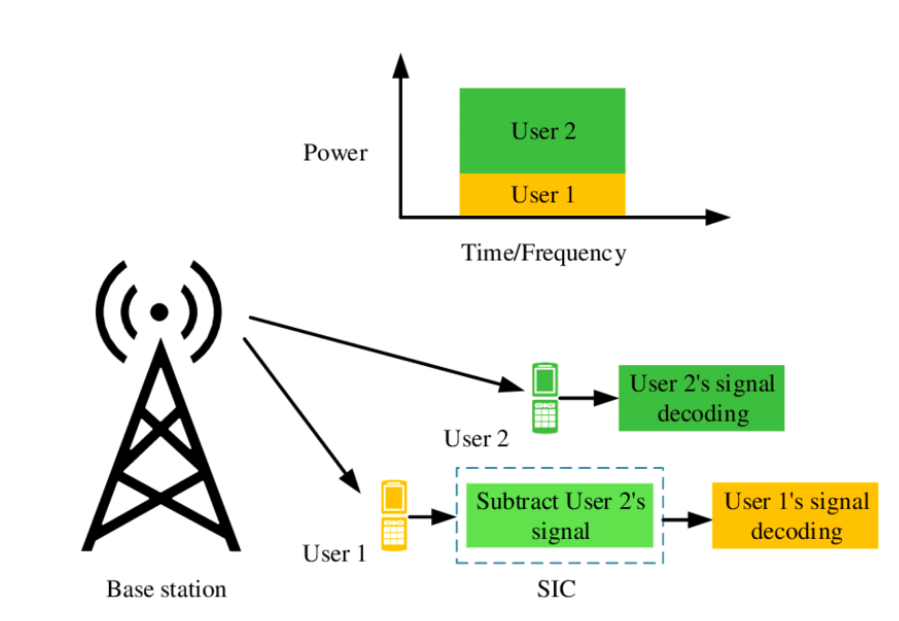
\includegraphics[width = 300pt, height = 220pt]{images/noma.png}
\end{figure}
\end{frame}

\begin{frame}{QAM symbol for $U_1$ and $U_2$}
    \begin{figure}
        \centering
        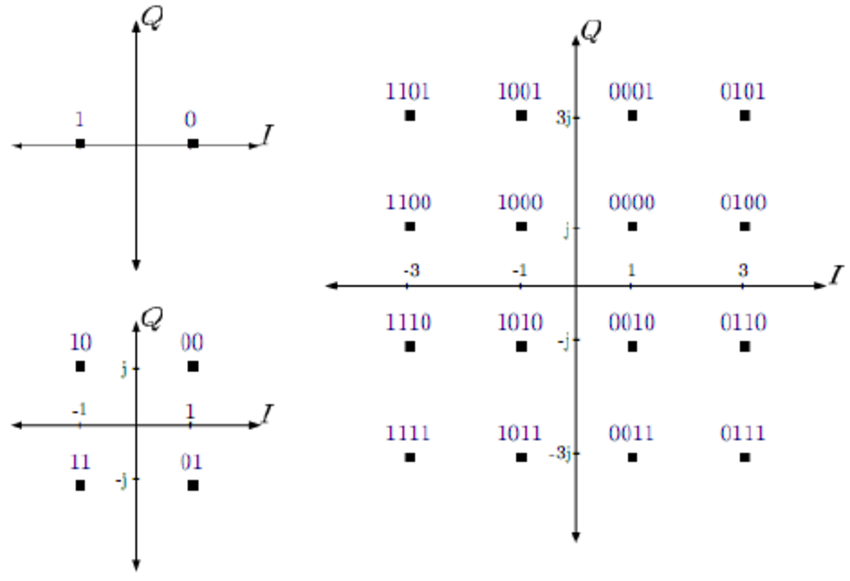
\includegraphics[width = 300pt, height = 220pt]{images/QAM_symbol.png}
    \end{figure}
\end{frame}

\begin{frame}{AWGN channel}
    Channel that adds noise to each transmitted symbol. The noise is complex normal $\sim$ CN(0, $N_o$)
    \begin{figure}
        \centering
        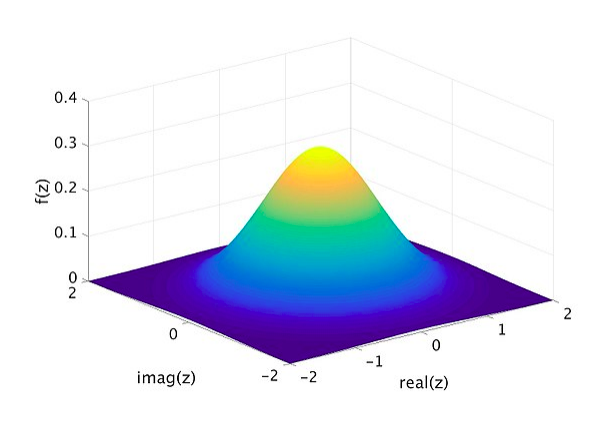
\includegraphics[width = 220pt, height = 180pt]{images/noise.png}
    \end{figure}
\end{frame}

\begin{frame}{NOMA symbol}
    \vspace{-0.5cm}
    \begin{align}
        Transmitted\; symbol(x) &= \sqrt{\beta_1 P_T}s_1 + \sqrt{\beta_2 P_T}s_2\\
        Received\; symbol(\hat{x}) &= h_n(\sqrt{\beta_1 P_T}s_1 + \sqrt{\beta_2 P_T}s_2) + CN(0, N_o)
    \end{align}
    \begin{figure}
        \centering
        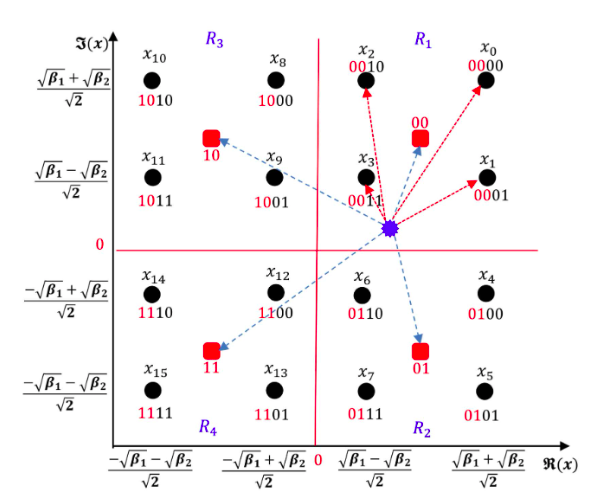
\includegraphics[width = 240pt, height = 180pt]{images/noma_symbol.png}
    \end{figure}
\end{frame}

\begin{frame}{BER for $U_1$}
    \begin{multline}
        P_{b_{1i}} = \dfrac{1}{\sqrt{M_1M_2}} \sum_{j = 0}^{\frac{1}{2}(\sqrt{M_1} - 1)} \sum_{k = 0}^{(\sqrt{M_2} - 1)} D_1(i,j)\\
        \times Q\left(\dfrac{h_1}{\sqrt{N_o}}\left[(2j+1)\sqrt{\beta_1P_T} + (2k - \sqrt{M_2} + 1)\sqrt{\beta_2P_T}\right]\right)
    \end{multline}
    \begin{equation}
        D_1(i,j) = (-1)^{\left \lfloor \frac{j2^{i-1}}{\sqrt{M_1}}\right \rfloor} \left(2^{i-1} - \left \lfloor\dfrac{j2^{i-1}}{\sqrt{M_1}} + \dfrac{1}{2} \right \rfloor\right)
    \end{equation}
    \begin{equation}
        BER = \dfrac{2}{log_2\sqrt{M_1}} \sum_{i=1}^{log_2\sqrt{M_1}} P_{b_{1i}}
    \end{equation}
\end{frame}

\begin{frame}{Results}
    \begin{figure}
        \centering
        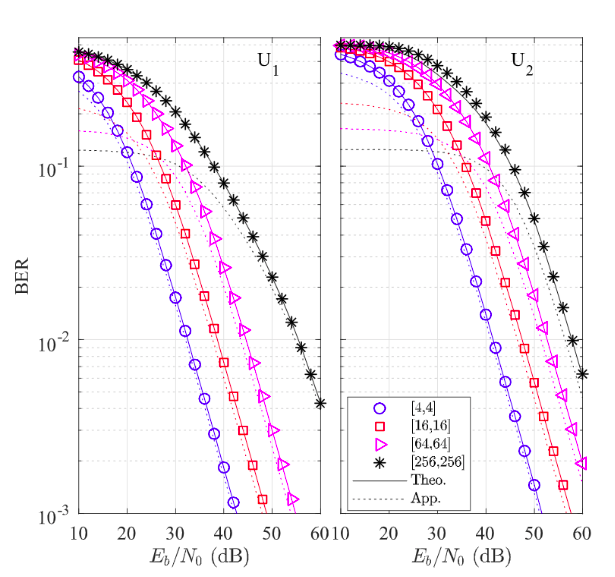
\includegraphics[width = 260pt, height = 220pt]{images/results.png}
    \end{figure}
\end{frame}
\end{document}
